\documentclass{article}
\usepackage{graphicx}
\usepackage{amsmath}
\usepackage{amsfonts}
\usepackage{bookmark}
\usepackage{booktabs}
\usepackage{exercises}
\graphicspath{ {./images/10.6} }
\usepackage{indentfirst}
\usepackage{amsthm}
\usepackage{yhmath}
\usepackage{geometry}
\usepackage{placeins}
\usepackage{csquotes}
\usepackage{pgfplots}
\newcommand*{\oldneg}{\mathord{\sim}}
\newcommand\showdiv[1]{\overline{\smash{)}#1}}
\newcommand\Mydiv[1]{%
\smash{\raise.3ex\hbox{$\big)$}}\mkern-8mu
        \overline{\enspace\strut#1}}
\setlength{\tabcolsep}{5pt}
\theoremstyle{definition}
\newtheorem{definition}{Definition}

\setlength{\parindent}{.5in}
\setlength{\parskip}{12pt}
\renewcommand{\arraystretch}{2}
\geometry{margin=1in}
\newcommand{\?}{\stackrel{?}{=}}
\pgfplotsset{width=7cm,compat=1.18}\usepgfplotslibrary{statistics}

\title{10.6 Answers}
\begin{document}
\maketitle

\section*{Derivations of the Sum and Difference Formulas}
We first derive the difference formula for cosine (which can be used to derive all of the other formulas).
We consider some angles $a$ and $b$ on the unit circle (as shown in the below diagram):\newline
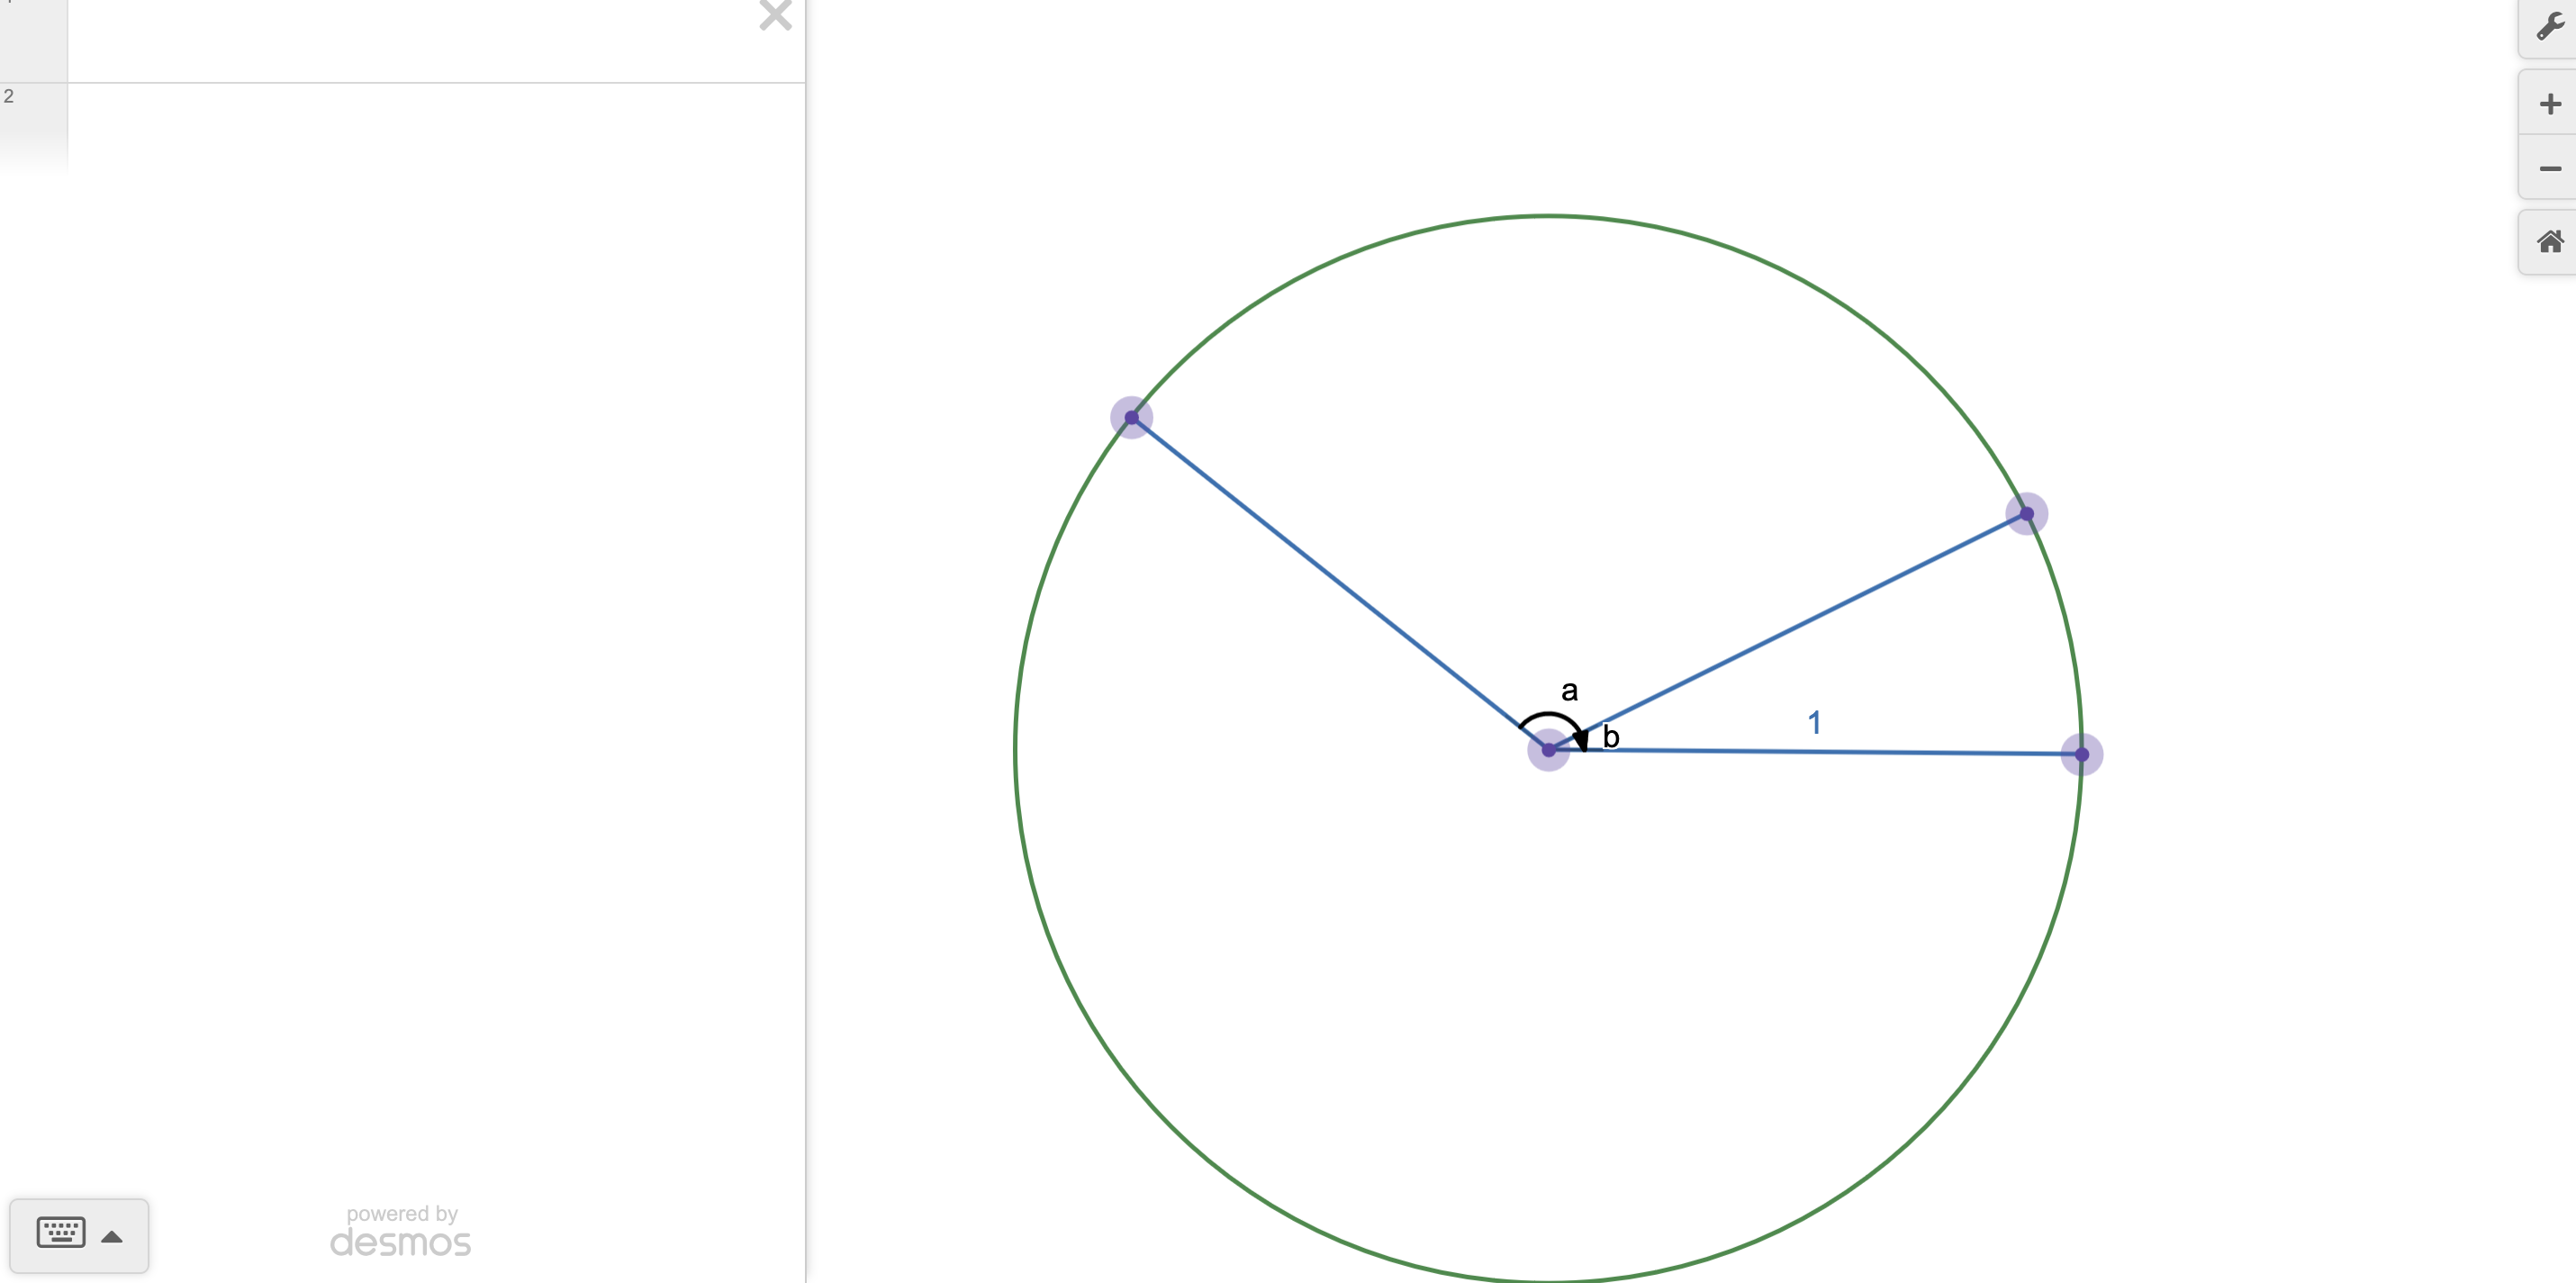
\includegraphics[width = 4in]{proof1}\newline
Angle $a$ intersects the unit circle at point $\cos a,\sin a$, and angle $b$ intersects the unit circle at 
point $\cos b,\sin b$. Consider the following diagram:\newline
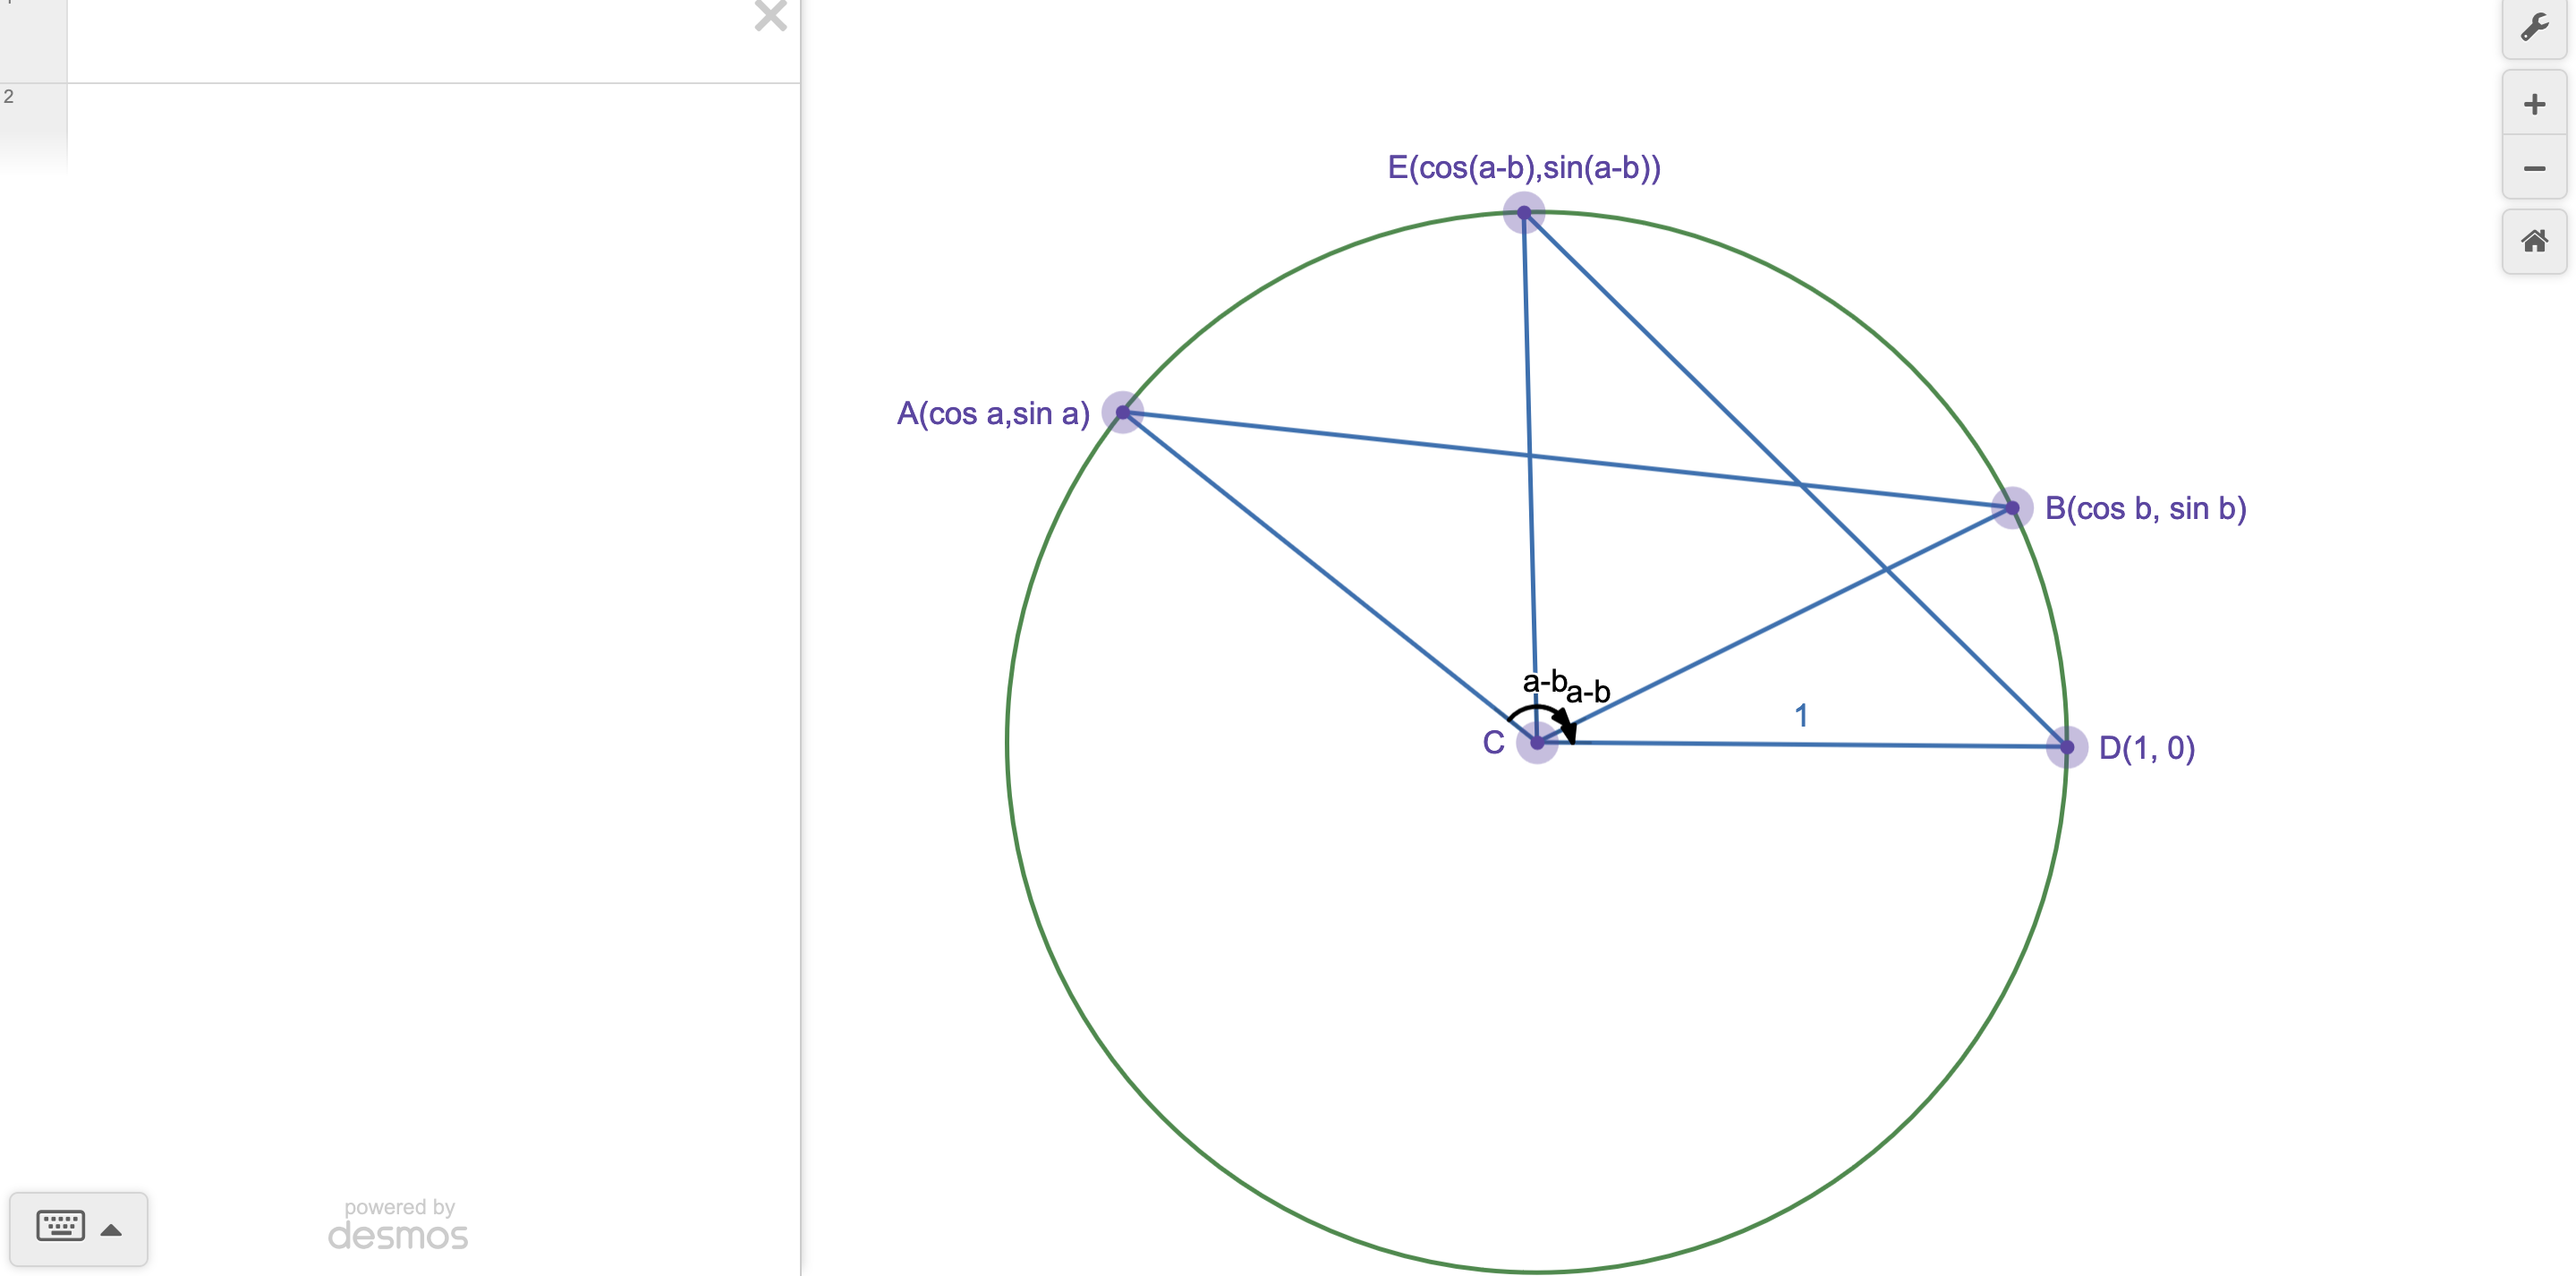
\includegraphics[width = 4in]{proof2}\newline
It shows $\triangle ACB$ and $\triangle ECD$, such that $\angle ACB=\angle ECD=a-b$. Now, we know that $\overline{AC}=\overline{EC}$ and 
$\overline{CB}=\overline{CD}$ (as they are all radii of the circle). Hence, by SAS, $\triangle ACB\equiv\triangle ECD$. This means
$\overline{AB}=\overline{ED}$. Now, we can compute $AB$:
\[ \sqrt{(\cos a-\cos b)^2+(\sin a-\sin b)^2} \]
\[ =\sqrt{\cos^2 a+\cos^2 b-2\cos a\cos b+\sin ^2a+\sin^2 b-2\sin a\sin b} \]
\[ =\sqrt{2-2\cos a\cos b-2\sin a\sin b}\textrm{ By the Pythagorean Identity} \]
and we can also compute $ED$:
\[ \sqrt{(\cos(a-b)-1)^2+(\sin(a-b))^2} \]
\[ =\sqrt{\cos^2(a-b)+1-2\cos(a-b)+\sin^2(a-b)} \]
\[ =\sqrt{2-2\cos(a-b)}\textrm{ By the Pythagorean Identity} \]
and thus, because $AB=ED$,
\[ \sqrt{2-2\cos a\cos b-2\sin a\sin b}=\sqrt{2-2\cos(a-b)} \]
\[ 2-2\cos a\cos b-2\sin a\sin b=2-2\cos(a-b) \]
\[ \cos(a-b)=\cos a\cos b+\sin a\sin b \] 
therefore completing the proof. Note that this only proves the case where $a>b>0$. We know prove the other cases. First consider the case where $a=b$. 
Then $\cos(a-b)=\cos 0=1$. But also
\[ \cos a\cos b+\sin a\sin b=\cos 0\cos 0+\sin 0\sin 0 \]
\[ =1+0=1 \] Hence this case also holds. Now suppose that $b>a>0$. Then
\[ \cos(a-b)=\cos(-(b-a)) \]
\[ =\cos(b-a) \]
\[ =\cos b\cos a+\sin b\sin a \]
\[ =\cos a\cos b+\sin a\sin b \] which proves this case. Now we suppose that either $a<0$ or $b<0$ (or both). We can show that, for any 
two angles $m$ and $n$, if $m_1$ and $n_1$ are coterminal with $m$ and $n$ respectively, then $\cos(m_1-n_1)=\cos(m-n)$. Because 
$m_1$ and $n_1$ are coterminal with $m$ and $n$ respctively, $m_1=m+360k$ and $n_1=n+360j$ for some integers $j$ and $k$. Thus
\[ \cos(m_1-n_1)=\cos(m+360k-(n+360j)) \]
\[ =\cos(m-n+360(k-j)) \] which shows that $m_1-n_1$ is coterminal with $m-n$, meaning $\cos(m_1-n_1)=\cos(m-n)$. Now, because we assumed that 
either $a<0$ or $b<0$, it follows that both $a$ and $b$ are coterminal with some angles $\theta_1>0$ and $\theta_2>0$, respctively. By the above result, 
$\cos(a-b)=\cos(\theta_1-\theta_2)$, and thus
\[ \cos(a-b)=\cos(\theta_1-\theta_2) \]
\[ =\cos\theta_1\cos\theta_2+\sin\theta_1\sin\theta_2 \]
\[ =\cos a\cos b+\sin a\sin b \] This last line follows because $a$ and $b$ are coterminal with $\theta_1$ and $\theta_2$, respctively. This completes the proof of 
the formula.
From the difference formula for cosine, we can derive the sum formula for cosine:
\[ \cos(a+b)=\cos(a-(-b)) \]
\[ =\cos a\cos(-b)+\sin a\sin(-b) \]
\[ =\cos a\cos b-\sin a\sin b \]
We can then derive the sine sum formula:
\[ \sin(a+b)=\cos(\frac{\pi}{2}-(a+b)) \]
\[ =\cos((\frac{\pi}{2}-a)-b) \]
\[ =\cos(\frac{\pi}{2}-a)\cos b+\sin(\frac{\pi}{2}-a)\sin b \]
\[ =\sin a\cos b+\cos a\sin b \]
And then also the sine difference formula:
\[ \sin(a-b)=\sin a\cos(-b)+\cos a\sin(-b) \]
\[ =\sin a\cos b-\cos a\sin b \]
Lastly, we can derive the sum formula for tangent:
\[ \tan(a+b)=\dfrac{\sin(a+b)}{\cos(a+b)} \]
\[ =\dfrac{\sin a\cos b+\cos a\sin b}{\cos a\cos b-\sin a\sin b} \]
\[ =\dfrac{\frac{\sin a\cos b+\cos a\sin b}{\cos a\cos b}}{\frac{\cos a\cos b-\sin a\sin b}{\cos a\cos b}} \]
\[ =\dfrac{\frac{\sin a}{\sin b}+\frac{\sin b}{\cos b}}{1-\frac{\sin a}{\cos a}\frac{\sin b}{\cos b}} \]
\[ =\dfrac{\tan a+\tan b}{1-\tan a\tan b} \]
and then the difference formula for tangent:
\[ \tan(a-b)=\dfrac{\tan a+\tan(-b)}{1-\tan a\tan(-b)} \]
\[ =\dfrac{\tan a-\tan b}{1+\tan a\tan b} \]

\end{document}
